%\documentclass[handout,trans]{beamer}
%\documentclass{beamer}
\documentclass[handout]{beamer}
\mode<presentation>
\usepackage{beamerthemesplit}
\usepackage{hyperref}
\usepackage{color}
\usepackage{colortbl}
\usepackage{dcolumn}
\usepackage{verbatim} 
\newcolumntype{.}{D{.}{.}{3}}
%\usetheme{Berlin}
  \setbeamercovered{transparent}

\newcommand{\colorr}{ \color{red} }
\newcommand{\colorb}{ \color{blue} }
\newcommand{\colorg}{ \color{green} }
\newcommand{\colory}{ \color{yellow} }
\newcommand{\colorm}{ \color{magenta} }
\newcommand{\colorc}{ \color{cyan} }

\newcommand{\red}{\color{red}}
\newcommand{\black}{\color{black}}
\newcommand{\blue}{\color{blue}}




\usepackage{amsfonts}
\usepackage{amssymb}
\usepackage{amsmath}
\usepackage{mathpazo}
\usepackage{hyperref}
\usepackage{multimedia}

\setcounter{MaxMatrixCols}{10}




\title[Stressing Bank Profitability for Interest Rate Risk]
{Stressing Bank Profitability for Interest Rate Risk}
\author[Bolotnyy, Edge, \& Guerrieri]{Valentin Bolotnyy, Federal Reserve Board, \\  
                           \vspace{0.05in}Rochelle M. Edge, Federal Reserve Board, \\ 
                           \vspace{0.05in} and \\ 
                           \vspace{0.05in}Luca Guerrieri, Federal Reserve Board}
\date[8/2013]{July 8, 2013}

\begin{document}
%\AtBeginSubsection

\begin{frame}
  \titlepage
\end{frame}

\begin{frame}
\frametitle{Motivation} 
\begin{itemize}
\item \vspace{0.075in} Regular bank stress testing is one of the three complementary reforms made to U.S. capital regulation since the crisis.
\item \vspace{0.25in} There are two important parts of stress testing.
\begin{itemize}
\item \vspace{0.075in} Formulating scenarios that are stressful to banks
\item \vspace{0.075in} Developing models that are able to translate scenarios into income, losses, and \emph{pro-forma} capital.
\end{itemize}
\item \vspace{0.25in} It is important that stress tests are able to translate accurately scenarios into bank financial statement outcomes.
\begin{itemize}
\item \vspace{0.075in} We examine this question for models of bank net interest margins (NIMs). 
\end{itemize}
\end{itemize}
\end{frame}

\begin{frame}
\frametitle{Net interest margins (for the top 25 bank holding companies, assessed quarterly)}

\vspace{-0.15in}
\begin{eqnarray}\textsf{Net interest margins}\!\!\!\!&=&\!\!\!\!\frac{\textsf{Net interest income (NII)}}{\textsf{Interest bearing assets}} \nonumber \\
                \!\!\!\!&=&\!\!\!\!\frac{\textsf{Total interest income}-\textsf{Total interest expenses}}{\textsf{Interest bearing assets}}  \nonumber 
\end{eqnarray} 
\begin{center}
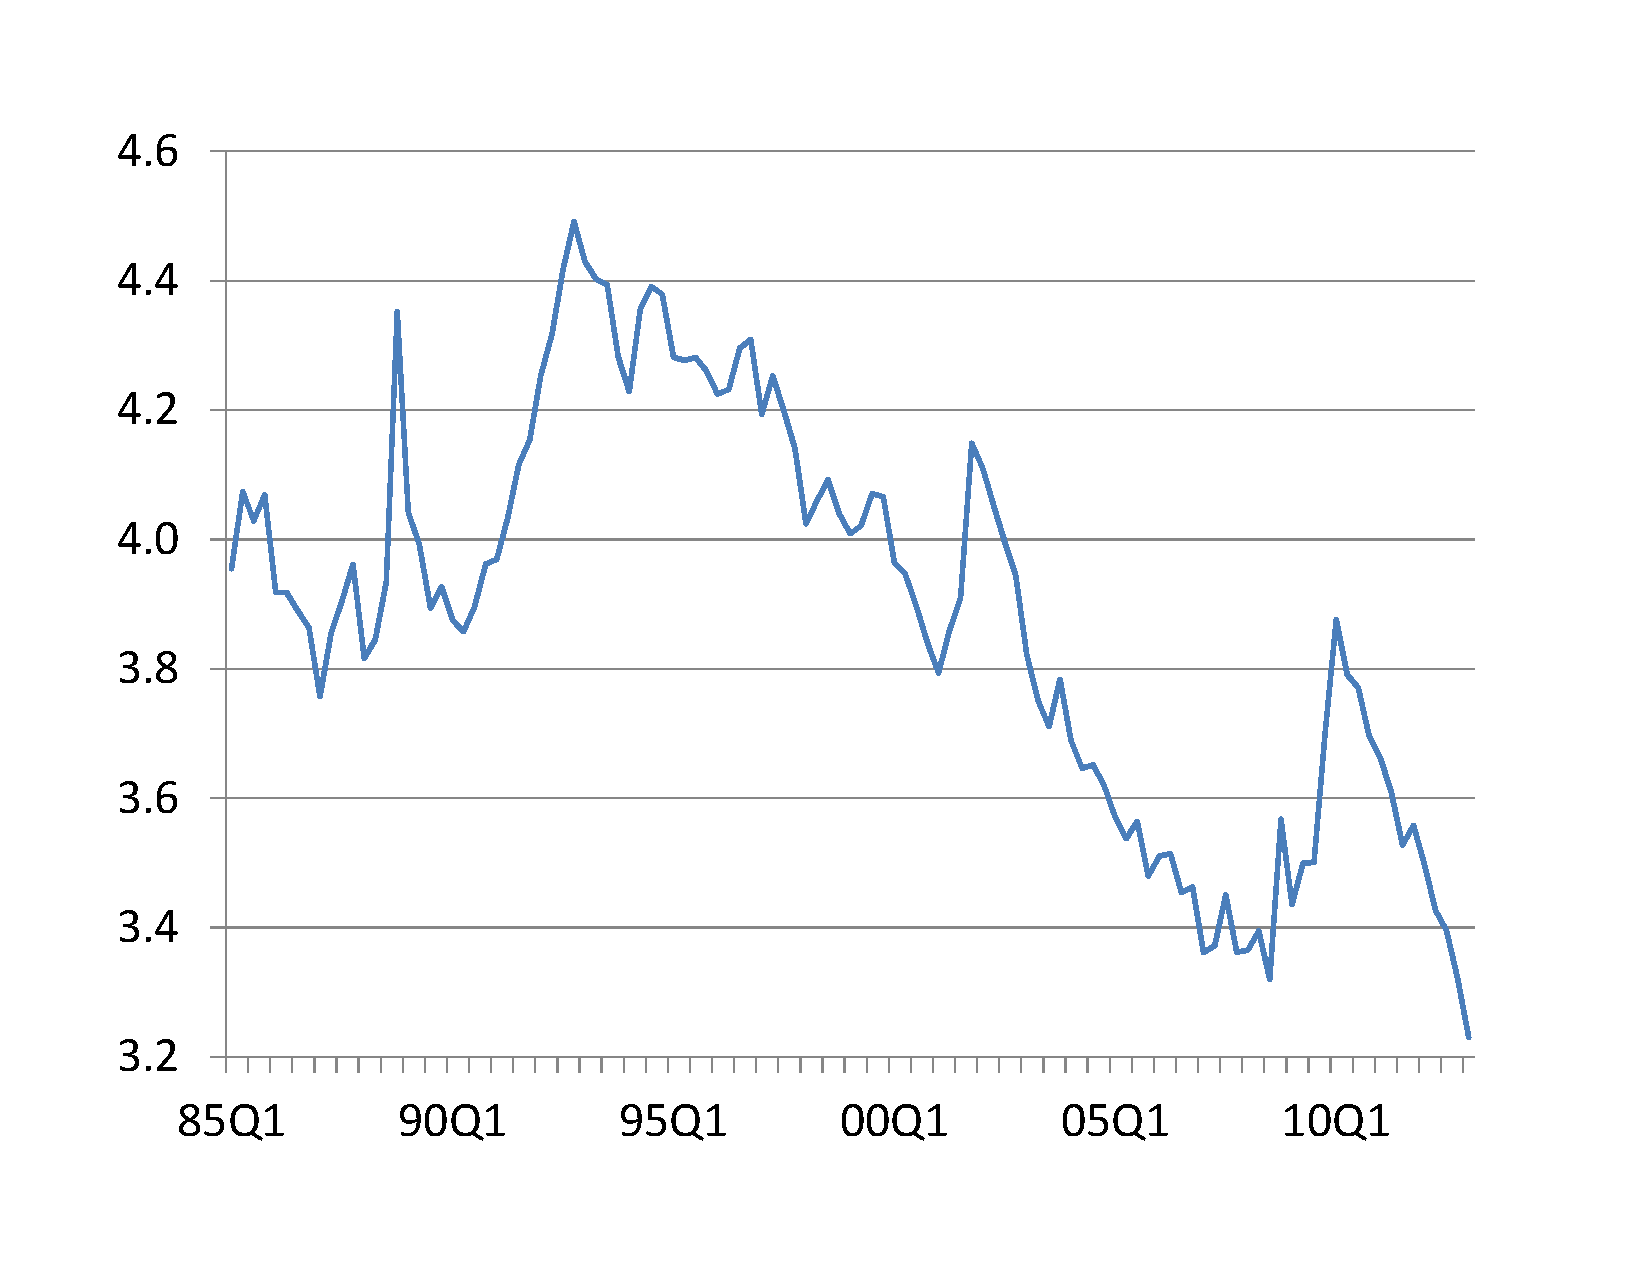
\includegraphics[height=5.4cm,width=7.2cm]{nims_crop.pdf}
\end{center}
%\begin{itemize}
%\item\vspace{0.0in} Net interest margins are our main variable of interest.
%\end{itemize}

\end{frame}


\begin{frame}
\frametitle{Why study NIMs} 
\begin{itemize}
\item \vspace{0.0in} Losses from banks' earning depressed or negative NII is an important source of risk to banks and the financial sector.
\item \vspace{0.1in} The U.S. savings and loans crisis was associated with NII and NIMs turning negative in the sector.
\end{itemize}
\begin{center}
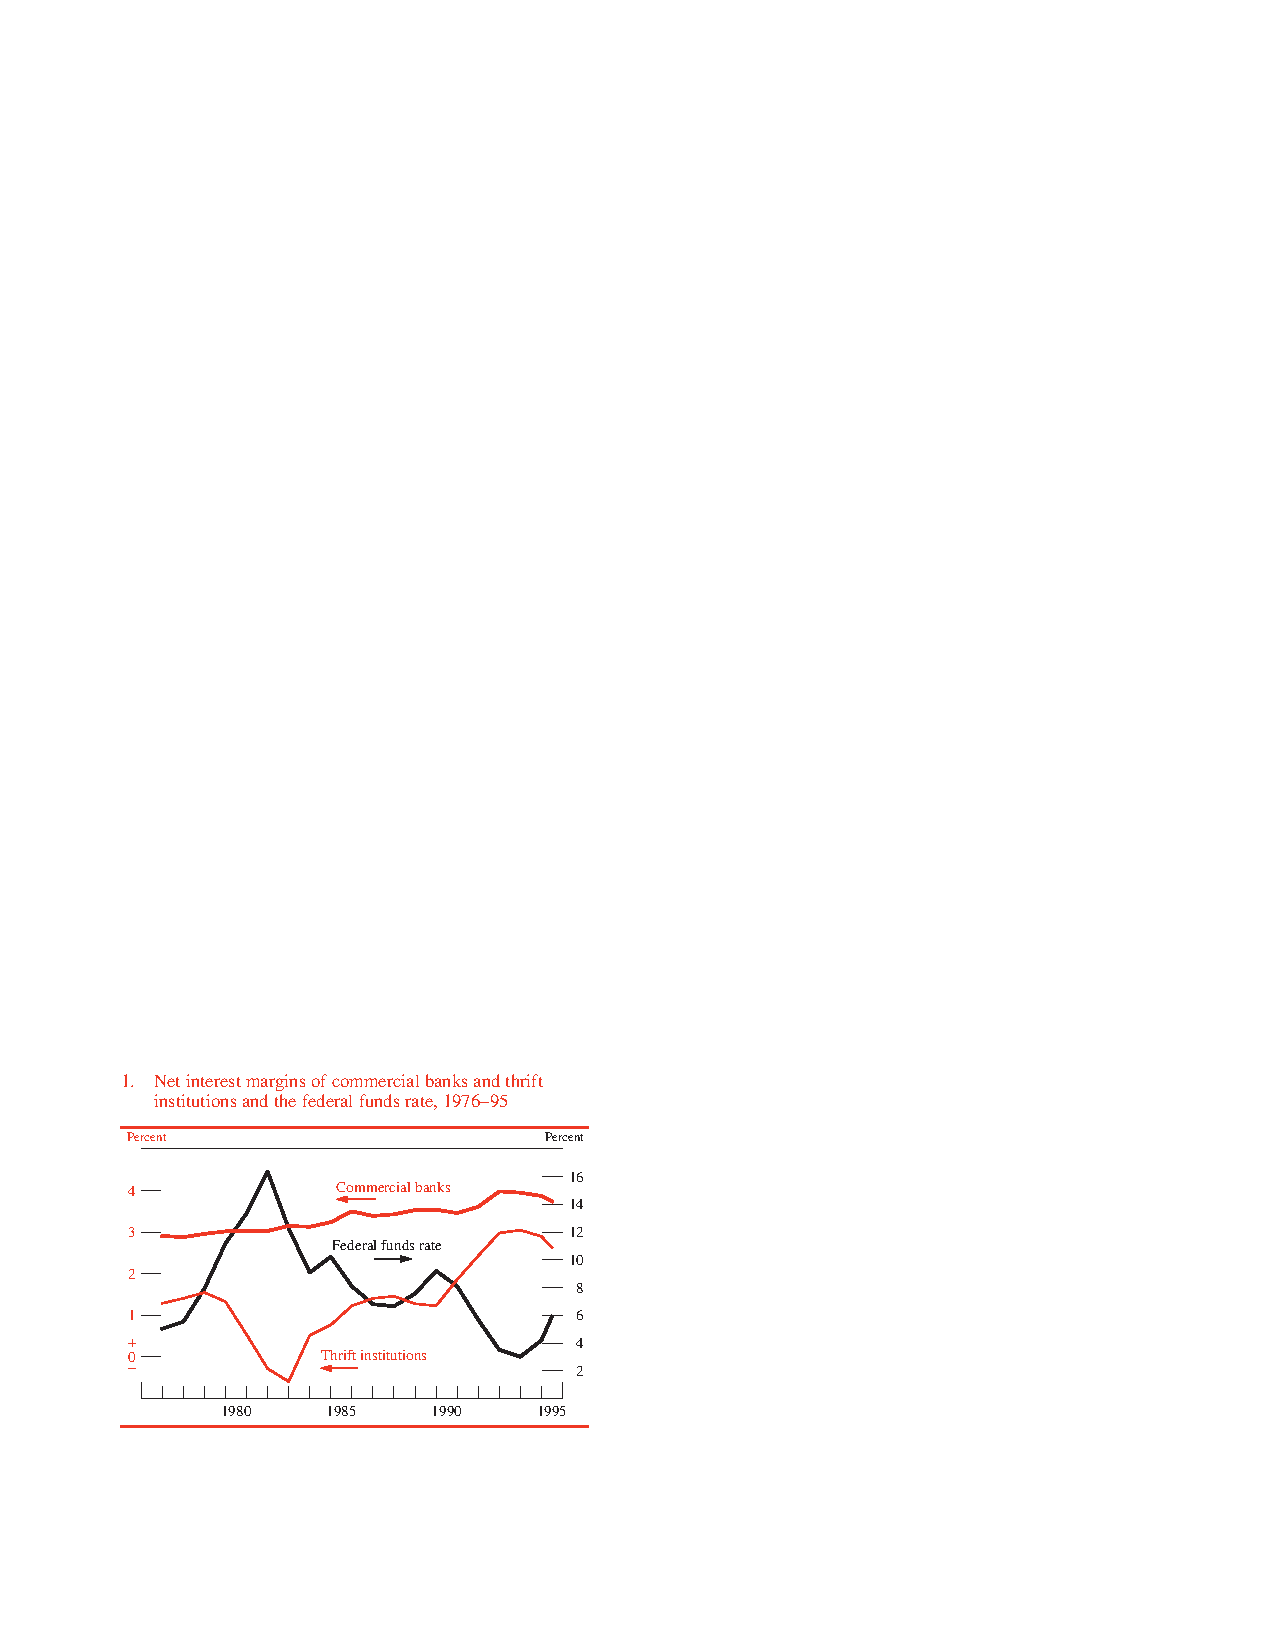
\includegraphics[height=4.4cm,width=5.9cm]{NIMs_Thrifts_CROP.pdf}
\end{center}
\vspace{-0.2in} \hspace{1.0in} {\tiny{Source: FR Bulletin, February 1996.}}\normalsize
\end{frame}

\begin{frame}
\frametitle{Why study NIMs, continued} 
\begin{itemize}
\item \vspace{0.0in} A few other banking crises have also been associated with depressed or negative NIMs; including,       
\begin{itemize}
\item \vspace{0.125in} The Nordic banking crises (in Finland, Sweden, and Norway) of the late 1980s/early 1990s; and, 
\item \vspace{0.125in} The U.K. secondary banking of 1973-75. 
\end{itemize}
\item \vspace{0.25in} NII is an important part of bank profitability.
\begin{itemize}
\item \vspace{0.125in} Bank equity analysis direct considerable attention to NII and NIMs in evaluating future bank profitability.
\item \vspace{0.125in} This reflects the fact that NII and NIMs are less volatile than other components of bank revenue.
\end{itemize}
\end{itemize}
\end{frame}

\begin{frame}
\frametitle{Objective of this paper}
\begin{itemize}
\item \vspace{0.0in} To develop a model that can be used to forecast bank net interest margins (NIMs). 
\end{itemize}
\vspace{-0.05in} 
\hspace{0.35in}\[\textsf{Net interest margins (NIMs)}=\frac{\textsf{Net interest income (NIIs)}}{\textsf{Interest bearing assets}} \] 
%\item \vspace{0.075in} $\textsf{Net interest margins (NIMs)} = 
%\frac{\textsf{Net interest income (NII)}}{\textsf{Interest bearing assets}}$ 
\begin{itemize}
\item \vspace{0.05in} We focus on conditional forecast performance.  
\begin{itemize}
\item \vspace{0.075in} Our interest is not in forecasting the macroeconomy (and especially not interest rates). 
\item \vspace{0.075in} Our interest is in forecasting bank profitability given the macroeconomy. 
\item \vspace{0.075in} Stress tests -- an important use of our model -- 
                       are conducted conditional on a set of macroeconomic scenarios.
\end{itemize}
\end{itemize}
\end{frame}

\begin{frame}
\frametitle{Key variables for modeling NIMs}
\begin{itemize}
\item \vspace{0.0in} The slope of the Treasury yield curve. 
\begin{itemize}
\item \vspace{0.05in} Reflects banks' return on maturity-transformation serivces -- one of the key services provided by banks.  
\end{itemize}
\item \vspace{0.1in} The level of short-term interest rates. 
\begin{itemize}
\item \vspace{0.05in} Indirectly reflects banks' return on transactions services -- another key service provided by banks.
\item \vspace{0.05in} The level of the short rate puts an upper limit on how much banks can earn from transactions services.  
\end{itemize}
\item \vspace{0.1in} The use of these variables is common in the macro-banking literature modeling NIMs.
\begin{itemize}
\item \vspace{0.05in} Kovner and Vickery (2012)
\item \vspace{0.05in} Covas, Rump, and Zakrajsek (2012)
\item \vspace{0.05in} English (2002)
\item \vspace{0.05in} English, Van den Heuvel, and Zakrajsek (2012)
\end{itemize}
\end{itemize}
\end{frame}

\begin{frame}
\frametitle{Key variables for modeling NIMs, continued}

\vspace{0.1in}\hspace{0.1in}
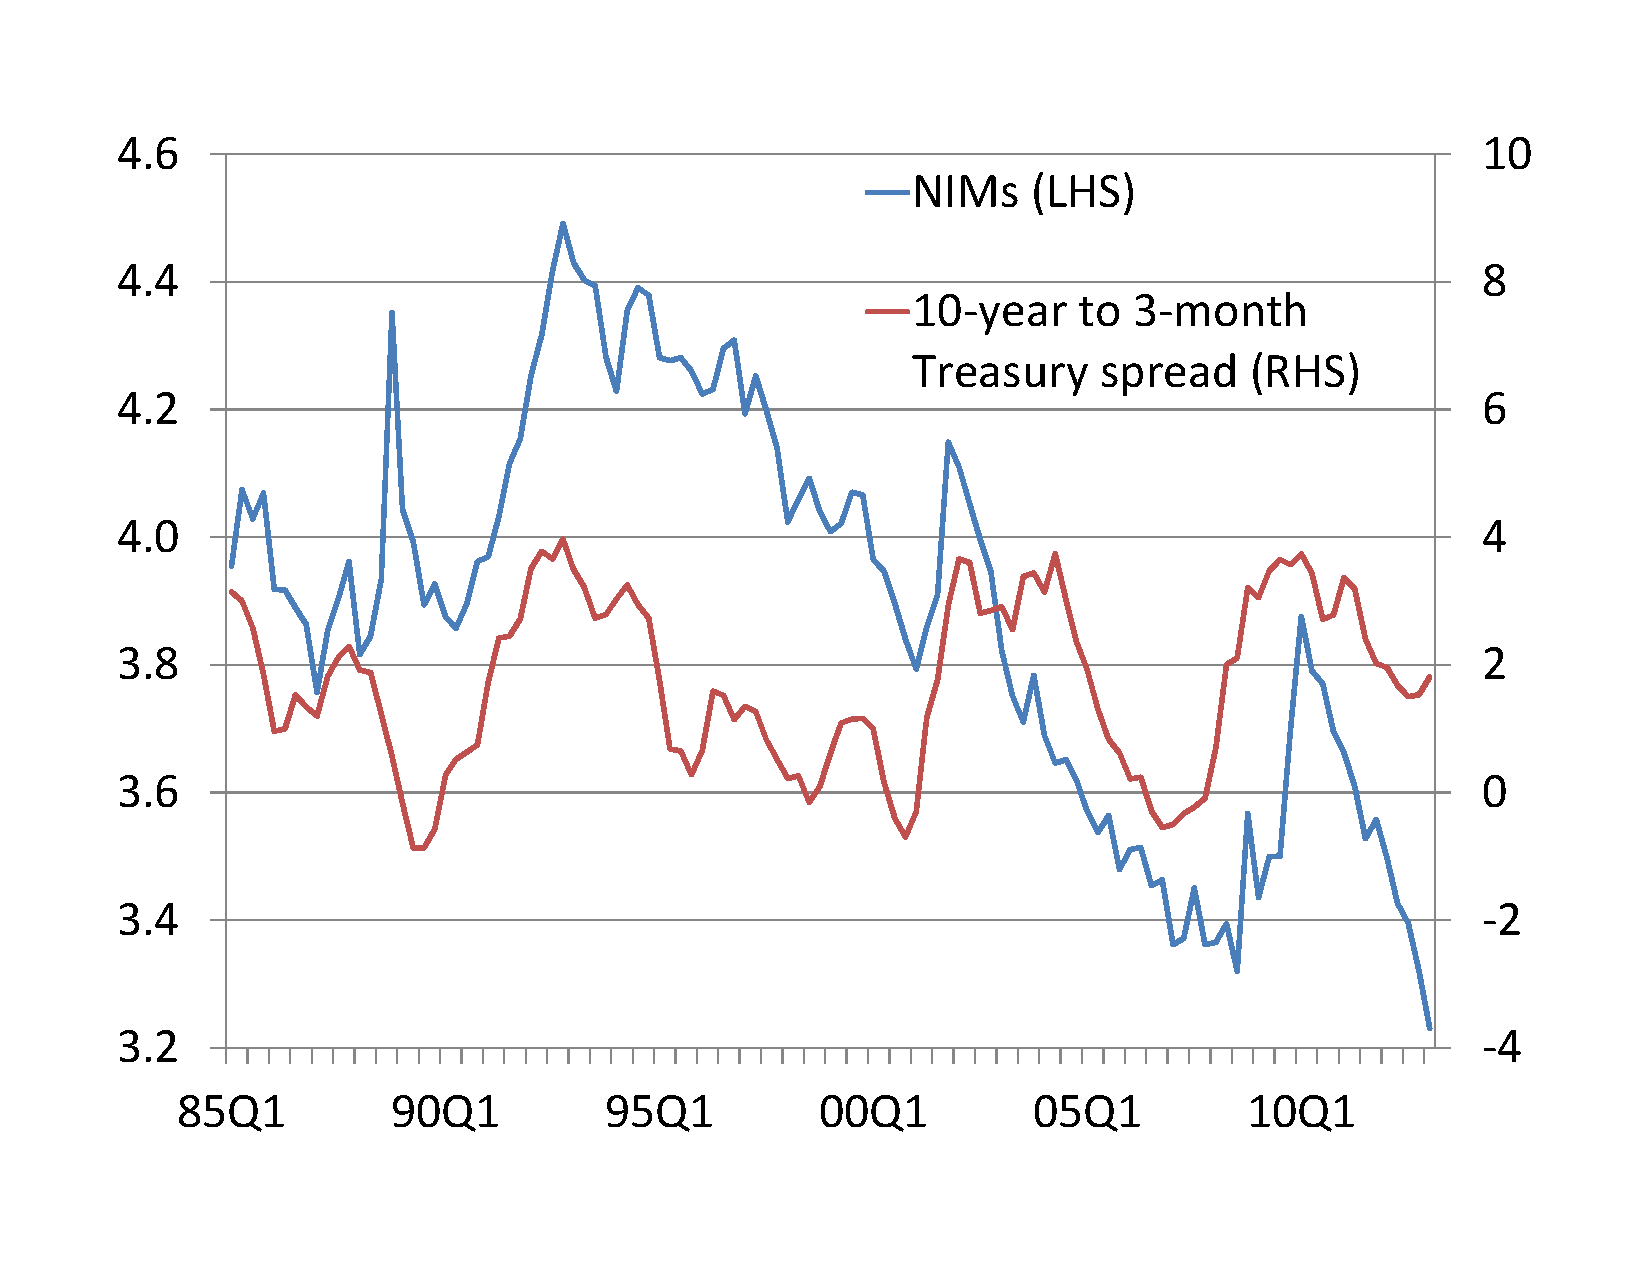
\includegraphics[height=3.6cm,width=4.8cm]{nims_slope_crop.pdf}  \hspace{0.25in}
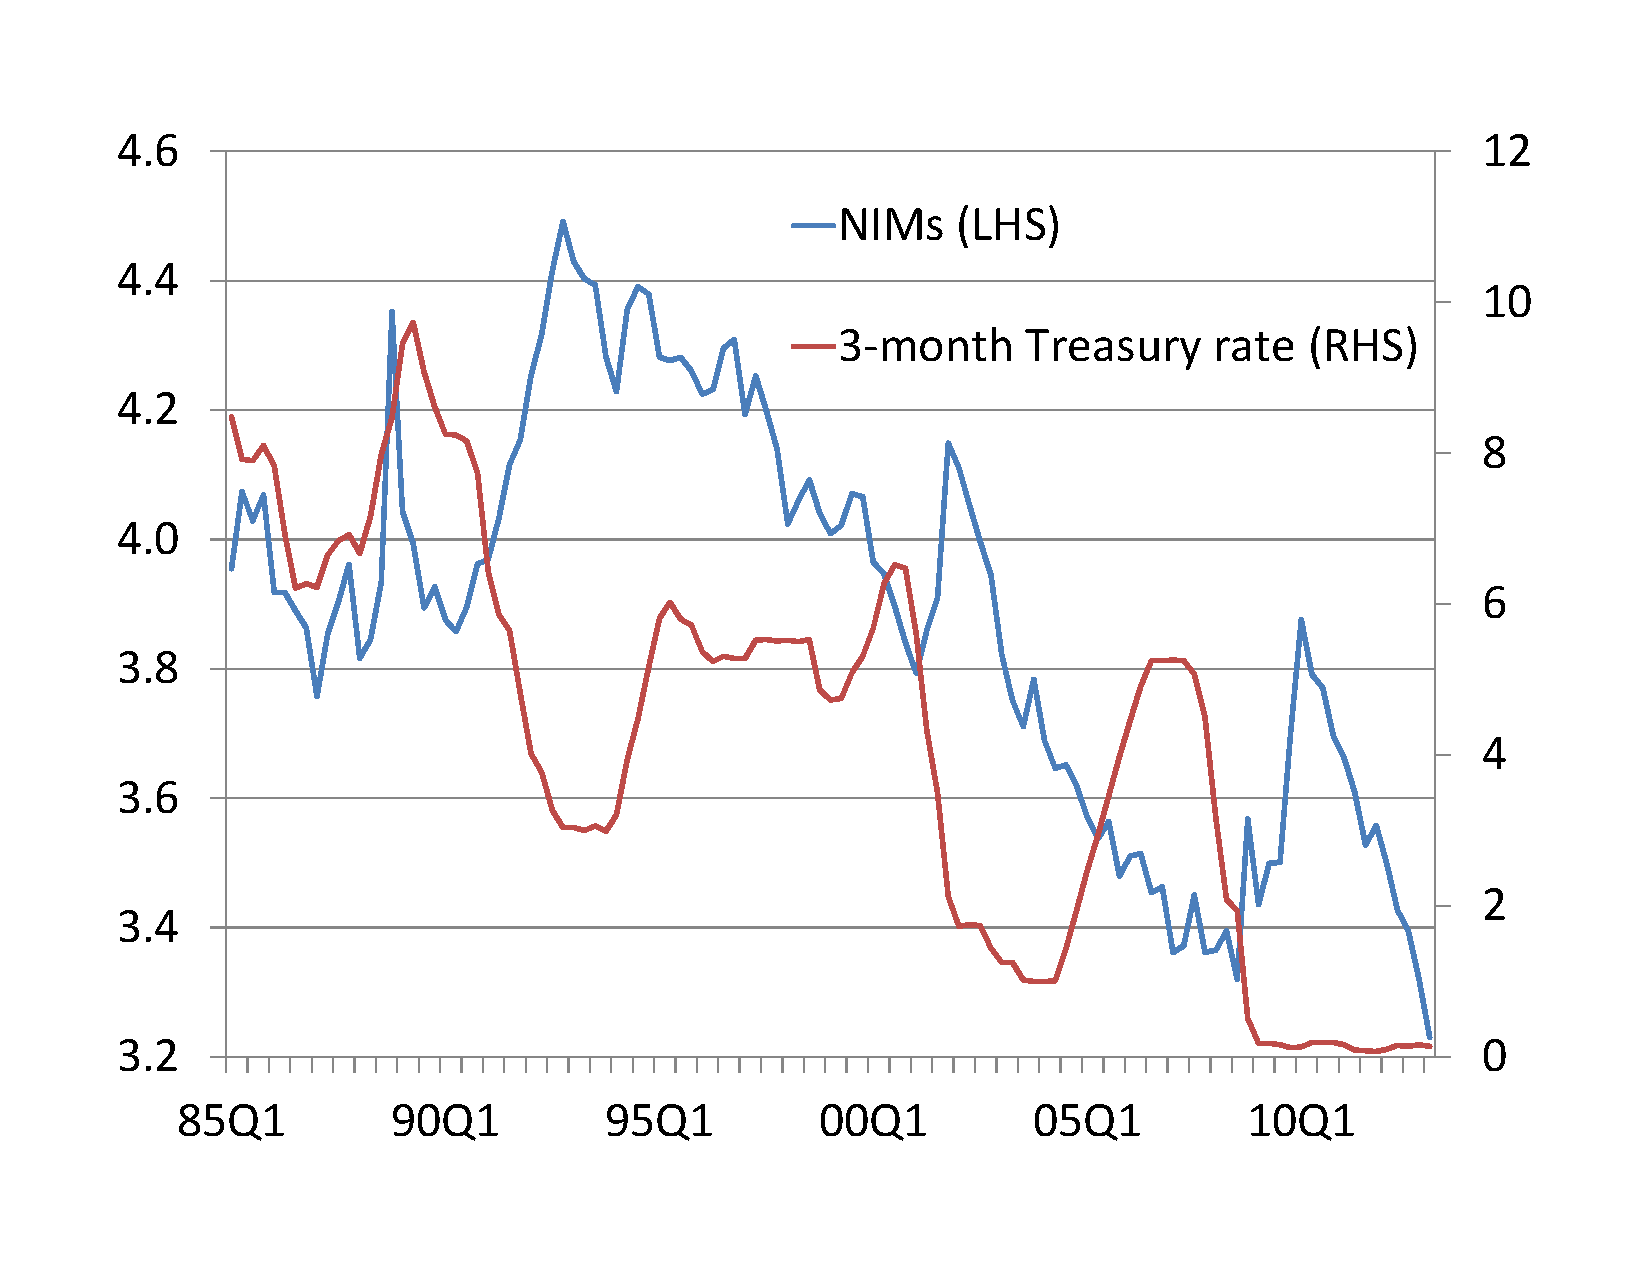
\includegraphics[height=3.6cm,width=4.8cm]{nims_level_crop.pdf}
\begin{itemize}
\item\vspace{0.1in} NIMs increase when the yield-curve steepens.
\begin{itemize}
\item \vspace{0.025in} Reflects the increased return to maturity transformation.
\end{itemize}
\item \vspace{0.075in} Changes in the short rate drive changes in the slope of the yield curve. 
\item \vspace{0.075in} There is an evident downward trend in the time series. 
\begin{itemize}
\item \vspace{0.025in} This may be tied to the lower level of interest rates.
\end{itemize}
\end{itemize}
\end{frame}

\begin{frame}
\frametitle{Key variables for modeling NIMs, continued}

%\begin{columns}[4cm]
%\column{7.2cm}
\vspace{0.1in}\hspace{0.65in}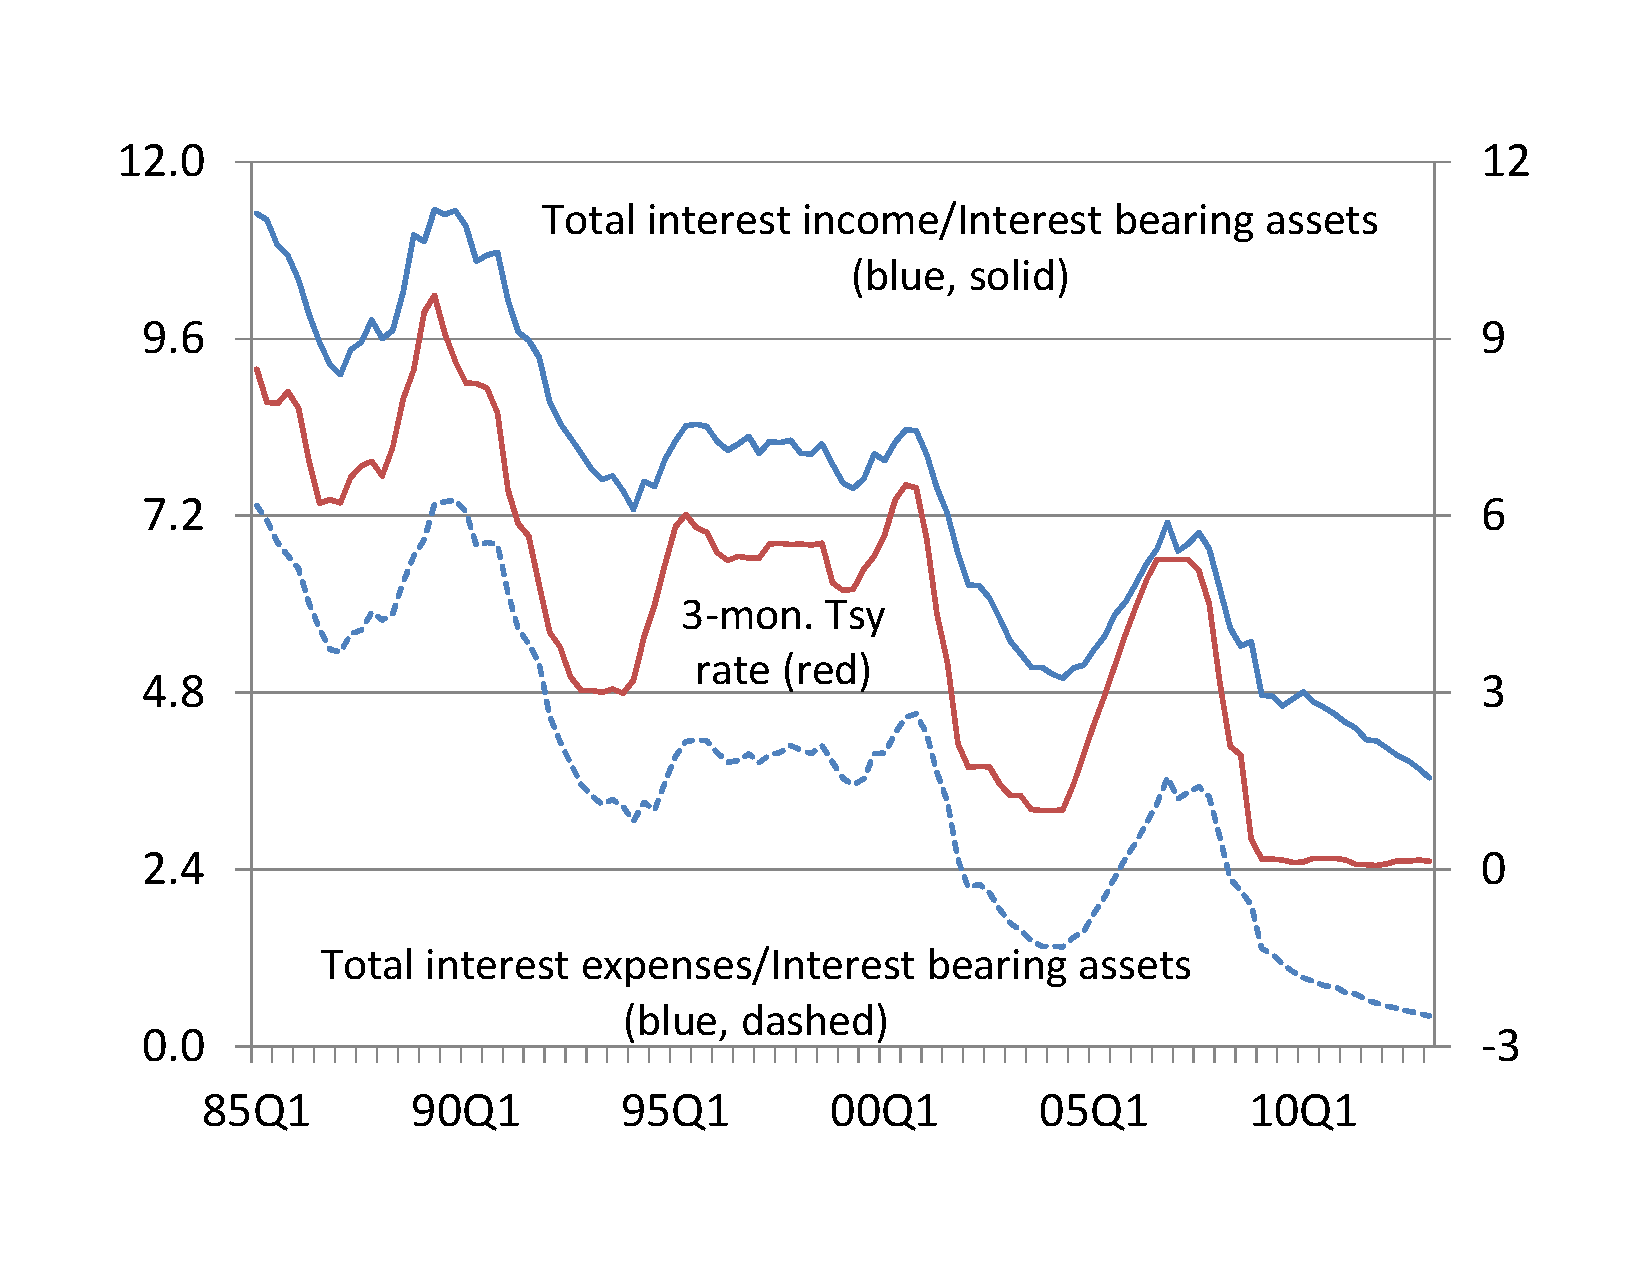
\includegraphics[height=5.4cm,width=7.2cm]{nims_components_crop.pdf}

%\column{4.8cm}
\begin{itemize}
\item\vspace{0.1in} The influence of the level of interest rates is evident in the two components of NIMs:
\begin{itemize}
\item \vspace{0.025in} Total interest income/Interest bearing assets; and,
\item \vspace{0.025in} Total interest expense/Interest bearing assets.
\end{itemize}
\end{itemize}
%\end{columns}
\end{frame}

\begin{frame}
\frametitle{Other key variables for modeling NIMs}
\begin{itemize}
\item \vspace{0.0in} The micro-banking literature on modeling NIMs emphasizes some different variables; such as,
\begin{itemize}
\item \vspace{0.05in} The degree of competition faced by banks in loan and deposit markets; and,
\item \vspace{0.05in} The volatility of interest rates.
\end{itemize}
\item\vspace{0.1in} The greater the degree of competition faced by banks in loan and deposit markets, 
\begin{itemize}
\item \vspace{0.05in} The lower the level of NIMs that banks can set. 
\end{itemize}
\item\vspace{0.1in} If banks are risk averse, the greater the volatility of interest rates,
\begin{itemize}
\item \vspace{0.05in} The more compensation for risk that banks will require to take deposits and make loans, and,
\item \vspace{0.05in} The higher the level of NIMs that banks will set. 
\end{itemize}
\end{itemize}
\end{frame}

\begin{frame}
\frametitle{Other key variables for modeling NIMs, continued}
\begin{itemize}
\item \vspace{0.15in} Relevant papers in the empirical micro-banking literature on modeling NIMs include:
\begin{itemize}
\item \vspace{0.15in} Ho and Saunders (1981) 
\item \vspace{0.15in} Angbazo (1997) 
\item \vspace{0.15in} Saunders and Schumacher (2000)
\end{itemize}

\end{itemize}
\end{frame}

\begin{frame}
\frametitle{Other key variables for modeling NIMs, continued}

\begin{columns}[4cm]

\column{7.2cm}
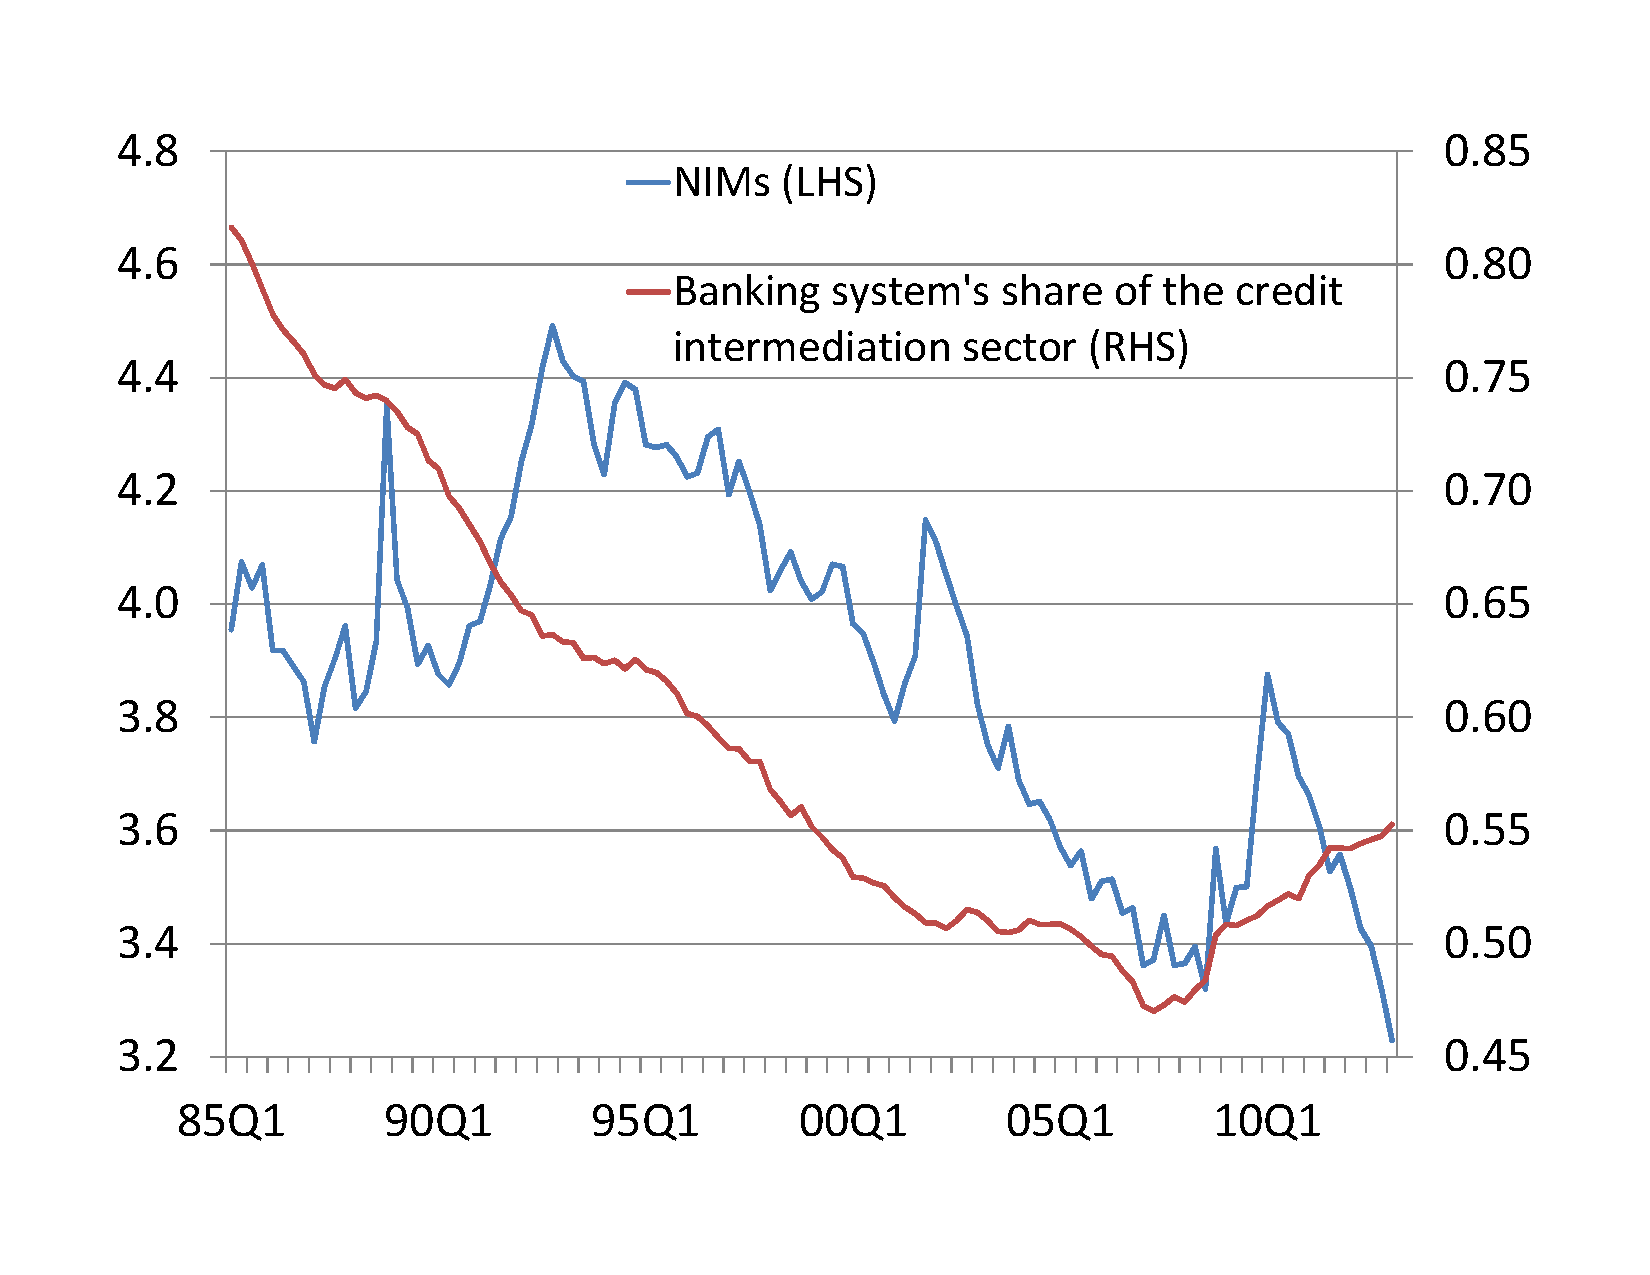
\includegraphics[height=5.4cm,width=7.2cm]{nims_competition_crop.pdf}

\column{4.8cm}
\begin{itemize}
\item\vspace{0.0in} The banking system's share of credit inter- mediation has shrunk.
\begin{itemize}
\item \vspace{0.05in} From 82\% in 1985 to 47\% in 2007.
\item \vspace{0.05in} It is now at 55\%.
\end{itemize}
\item \vspace{0.125in} Competition from the shadow banking sector has put pressure on deposit and loan rates.
\item \vspace{0.125in} One other variable we have not yet considered is interest rate volatility.
\end{itemize}
\end{columns}
\end{frame}

\begin{frame}
\frametitle{Net interest margins:  A few quirks in the data}

\begin{columns}[4cm]

\column{7.2cm}
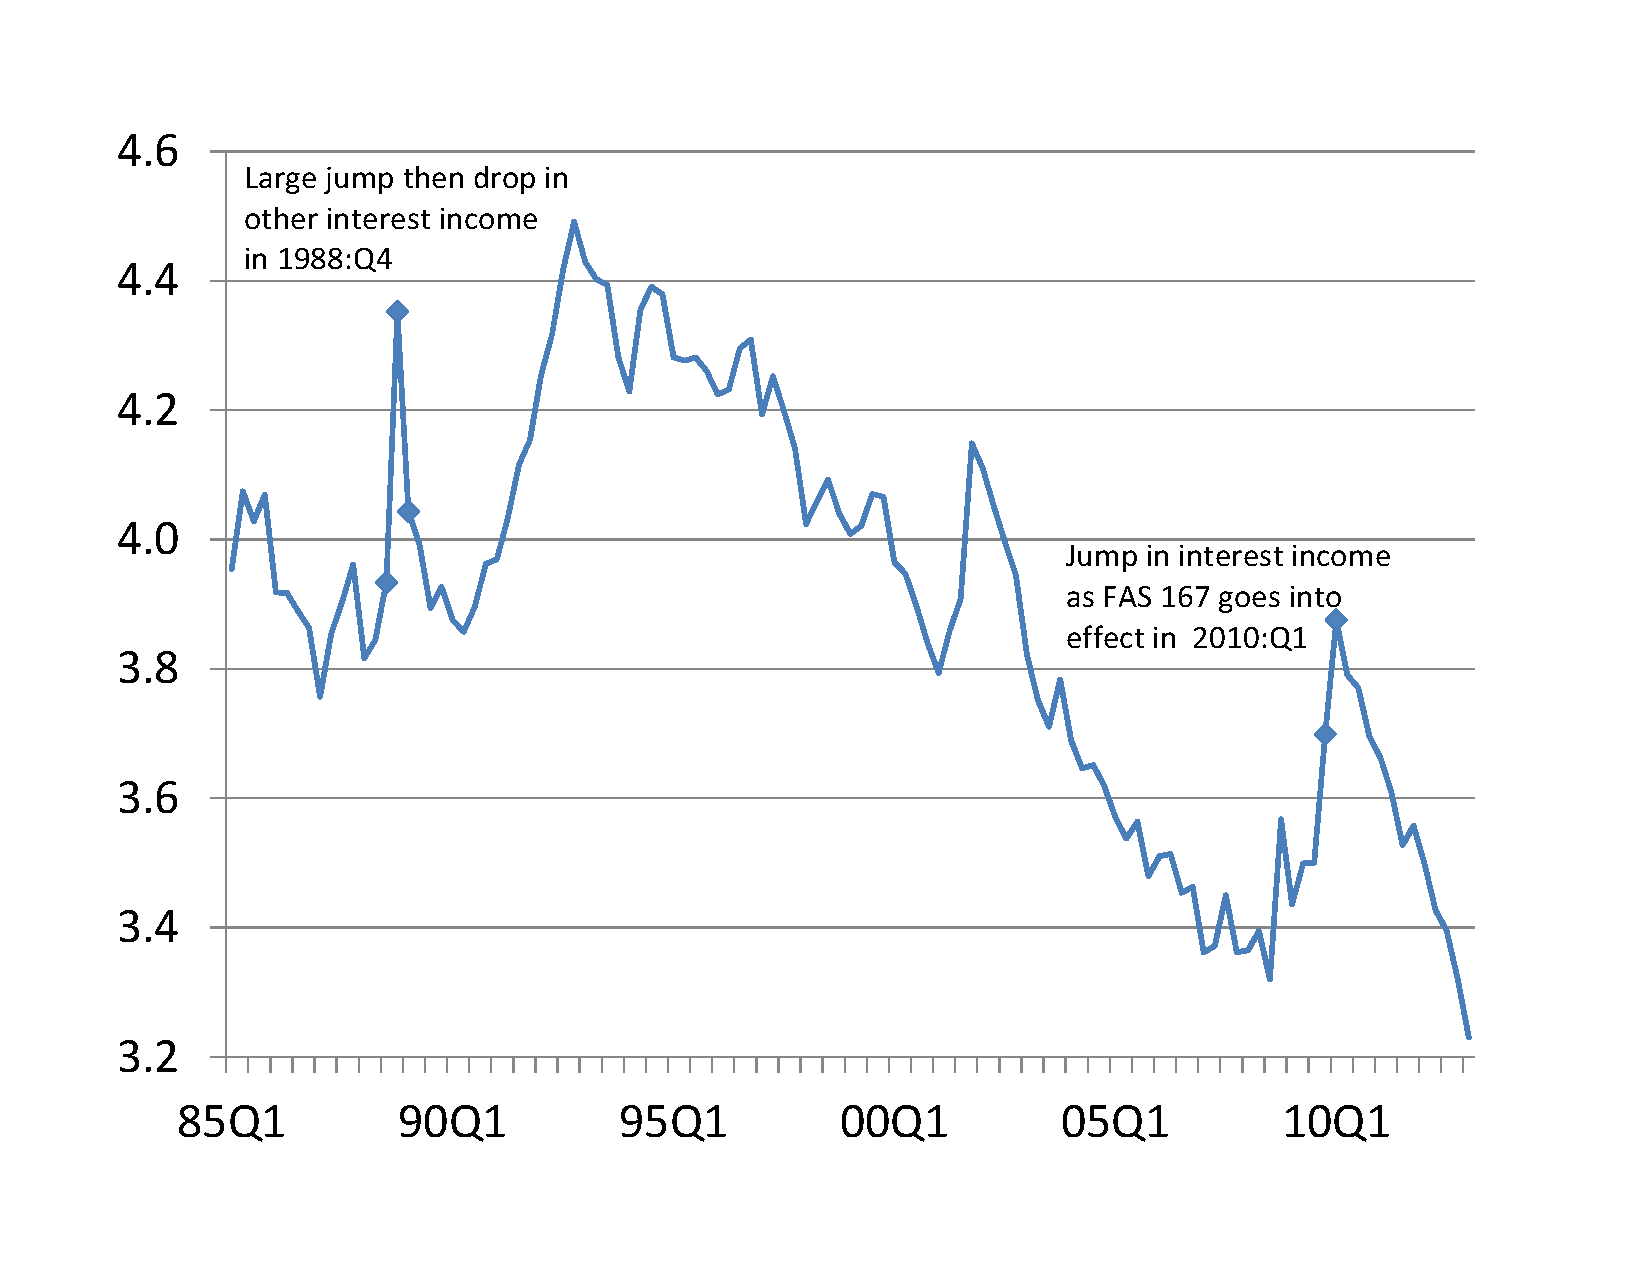
\includegraphics[height=5.4cm,width=7.2cm]{nims_bugs_crop.pdf}

\column{4.8cm}
\begin{itemize}
\item\vspace{-0.15in} The spike in 1988:Q4 reflects a jump then drop in ``other'' interest income.
\begin{itemize}
\item \vspace{0.075in} This reflects interest from Brazil overdue since early 1987.
\end{itemize}
\item \vspace{0.15in} The jump in 2010:Q1 reflects FAS 167 going into effect. 
\begin{itemize}
\item \vspace{0.075in} We will adjust for this jump.
\end{itemize}
\end{itemize}
\end{columns}
\end{frame}

\begin{frame}
\frametitle{Forecasting models} 

We are interesting in comparing the pseudo-out-of-sample forecasting performance of different models:
\begin{enumerate}
\item Forecast combination based on yields
\item Dynamic factor model
\item Dynamic factor model with second-step regression
\item Principal Component Regression based on yields
\item Partial Least Squares based on yields
\item Forecast combination based on observed yield-curve factors
\item A VAR with observed yield curve factors
\item A random walk without a drift
\end{enumerate}
\end{frame}

\begin{frame}
\frametitle{What's next}
\begin{itemize}

\item Next -- We describe each of the models in our horse race

\item We focus on the baseline specification for each model 

\item Each model can be extended to include additional variables (sensitivity analysis)

\end{itemize}
\end{frame}

\begin{frame}

\frametitle{1. Forecast Combination Based on Yields }
We regress NIMs on each yield $r(\tau )_{t-1}$ separately: \
\begin{equation*}
NIM_{t}=c_{\tau }+\rho _{\tau }NIM_{t-1}+\gamma _{\tau }r(\tau )_{t-1}+{\eta
_{\tau ,t}}
\end{equation*}

Each regression is used to produce a recursive $s$ step-ahead forecast of NIMs
conditional on yields on treasuries with maturity $\tau $ observed through
period $t+s-1.$ This conditional forecast is denoted by $NIM_{\tau ,t+s/t}.$%
The simple forecast combination is then given by:%
\begin{equation*}
NIM_{t+s/t}=\sum_{\tau }\frac{NIM_{\tau ,t+s/t}}{N},
\end{equation*}%
where $N$ is the number of maturities considered.

\end{frame}

\begin{frame}
\frametitle{2. A Dynamic Factor Model}
Using the state space
representation, the state equations of our dynamic factor model
is given by
\begin{equation*}
\left(
\begin{array}{c}
{L_{t+1}-\mu _{L}} \\
{S_{t+1}-\mu _{S}} \\
{C_{t+1}-\mu _{C}} \\
\widehat{NIM}_{t+1}-\mu _{\widehat{NIM}}%
\end{array}%
\right) {\normalsize \ =\ }\left(
\begin{array}{cccc}
a_{11} & a_{12} & a_{13} & 0 \\
a_{21} & a_{22} & a_{23} & 0 \\
a_{31} & a_{32} & a_{33} & 0 \\
a_{41} & a_{42} & a_{43} & a_{44}%
\end{array}%
\right) {\normalsize \ }\left(
\begin{array}{c}
{L_{t}-\mu _{L}} \\
{S_{t}-\mu _{S}} \\
{C_{t}-\mu _{C}} \\
\widehat{NIM}_{t}-\mu _{\widehat{NIM}}%
\end{array}%
\right) {\normalsize +}\left(
\begin{array}{c}
{\eta _{Lt}} \\
{\eta _{St}} \\
{\eta _{Ct}} \\
{\eta _{NIMt}}%
\end{array}%
{\normalsize \ }\right) ,
\end{equation*}

$L_{t},S_{t},$ and $C_{t}$ are level slope and curvature factors for
the yield curve, respectively, and $\widehat{NIM}_{t}$ represent a measure
of NIMs cleaned of observation error. 

The term $\mu _{x}$ denotes the mean
of $x$. The terms ${\eta _{Lt}}$, ${\eta _{St}}$, ${\eta _{Ct}}$, ${\eta
_{NIMt}}$ denote independently distributed innovations with joint covariance
matrix $\Omega $.

\end{frame}

\begin{frame}
\frametitle{2. A Dynamic Factor Model -- Observation Equation}

The observation equations for yields on treasuries of maturity $\tau $ take the form:
\begin{equation*}
r(\tau )=\left(
\begin{array}{cccc}
1 & \frac{1-e^{-\lambda \tau }}{\lambda \tau } & \frac{1-e^{-\lambda \tau }}{%
\lambda \tau }-e^{-\lambda \tau } & 0%
\end{array}%
\right) \left(
\begin{array}{c}
{L_{t}-\mu _{L}} \\
{S_{t}-\mu _{S}} \\
{C_{t}-\mu _{C}} \\
\widehat{NIM}_{t}-\mu _{\widehat{NIM}}%
\end{array}%
\right) +e(\tau )_{t},
\end{equation*}%
The observation equation for NIMs takes the form:
\begin{equation*}
NIM_{t}=\left(
\begin{array}{cccc}
0 & 0 & 0 & 1%
\end{array}%
\right) \left(
\begin{array}{c}
{L_{t}-\mu _{L}} \\
{S_{t}-\mu _{S}} \\
{C_{t}-\mu _{C}} \\
\widehat{NIM}_{t}-\mu _{\widehat{NIM}}%
\end{array}%
\right) +e(NIM)_{t},
\end{equation*}

Out-of-sample conditional forecasts for NIMs from this model, are obtained
using the Kalman filter.

\end{frame}

\begin{frame}

\frametitle{3. Dynamic Factor Model with Second-Step Regression}

First, we estimate the level, slope, and curvature factors in isolation:
\begin{equation*}
\left(
\begin{array}{c}
{L_{t+1}-\mu _{L}} \\
{S_{t+1}-\mu _{S}} \\
{C_{t+1}-\mu _{C}}%
\end{array}%
\right) {\normalsize \ =\ }\left(
\begin{array}{ccc}
a_{11} & a_{12} & a_{13} \\
a_{21} & a_{22} & a_{23} \\
a_{31} & a_{32} & a_{33}%
\end{array}%
\right) {\normalsize \ }\left(
\begin{array}{c}
{L_{t}-\mu _{L}} \\
{S_{t}-\mu _{S}} \\
{C_{t}-\mu _{C}}%
\end{array}%
\right) {\normalsize +}\left(
\begin{array}{c}
{\eta _{Lt}} \\
{\eta _{St}} \\
{\eta _{Ct}}%
\end{array}%
\right)
\end{equation*}

\begin{equation*}
r(\tau )=\left(
\begin{array}{ccc}
1 & \frac{1-e^{-\lambda \tau }}{\lambda \tau } & \frac{1-e^{-\lambda \tau }}{%
\lambda \tau }-e^{-\lambda \tau }%
\end{array}%
\right) \left(
\begin{array}{c}
{L_{t}-\mu _{L}} \\
{S_{t}-\mu _{S}} \\
{C_{t}-\mu _{C}} 
\end{array}%
\right) +e(\tau )_{t},
\end{equation*}

We obtain smoothed estimates of the factors $L_{t},S_{t},$ and $C_{t}$
conditional on information up until period $T.$ 
\end{frame}

\begin{frame}

\frametitle{3. Dynamic Factor Model with Second-Step Regression -- Continued }

{\blue Alternative a.}  A multivariate regression
\begin{equation*}
NIM_{t}=c+\rho NIM_{t-1}+\gamma _{L}L_{t-1}+\gamma _{S}S_{t-1}+\gamma
_{C}C_{t-1}
\end{equation*}

{\blue Alternative b.}  Forecast Combination (each factor included in a
separate equation and forecasts from each equation combined) 
\begin{equation*}
NIM_{t}=c_{i}+\rho _{i}NIM_{t-1}+\gamma _{i}F_{i,t-1}+{\eta _{i,t},}
\end{equation*}%
where $F_{i}\in \left\{ L,S,C\right\} .$ Forecasts $NIM_{i,t+s/t}$ from each
separate regression are then aggregated as:
\begin{equation*}
NIM_{t+s/t}=\sum_{i}\frac{NIM_{i,t+s/t}}{3}.
\end{equation*}

\end{frame}

\begin{frame}
\frametitle{4. Principal Component Regression}

\begin{itemize}
\item Let $X$ a $T \times n$ matrix of $n$ Treasury yields.  Using the spectral decomposition, one obtains $X'X = VDV'$.

\item Let $V_i$ be the eigenvector corresponding to $i^{th}$ largest eigenvalue.

\item The $i^{th}$ principal component is defined as $PC_i = XV_i$.

\item We estimate:
\begin{equation*}
NIM_t = c + \rho NIM_{t-1} + \sum_{i=1}^3 \gamma_i PC_{i,t-1}. 
\end{equation*}
\end{itemize}

\end{frame}


\begin{frame}

\frametitle{5. Partial Least Squares}

\begin{itemize}
\item Partial least squares is a compression technique analogous to principal components.
\item Project the regressors onto a lower dimensional space. 
\item Each new regressor is a linear combination of the original regressors.
\item What distinguishes PLS from PCR is how the
projection is done.
\item In particular, PCR chooses basis vectors of its low
dimensional projection to describe as much as
possible the variation in the data $X$.
\item However nothing guarantees that the principal
components, which �explain� $X$ optimally, will be
relevant for the prediction of $Y$.
\item Solution: incorporate information from $Y$ when
choosing the projection (use SVD of $X'Y$).

\end{itemize}
\end{frame}

\begin{frame}
\frametitle{5. Partial Least Squares -- continued}

Choose X to include 
\begin{itemize}
\item Lagged NIM
\item Yields 
\end{itemize}

Focus on PLS with 4 factors.

\end{frame}

\begin{frame}
\frametitle{6. Forecast Combination Based on Observed Factors }

\begin{itemize}
\item Define $\left\{
L,S,C\right\}$ the observed factors as:

$L = \frac{r(3m) + r(2yr) + r(10yr)}{3}$

$S = r(3m)-r(2yr)$

$C = \left[ r(3m)-r(2yr) \right] - \left[ r(2yr)-r(10yr) \right]$

\item Consider
\begin{equation*}
NIM_{i,t}=c_{i}+\rho _{i}NIM_{t-1}+\gamma _{i}O_{i,t-1}+{\eta _{i,t},}
\end{equation*}%
where $O_{i}\in \left\{ L,S,C\right\} .$ 

\item Forecasts  from each separate
regression, $NIM_{i,t+s/t}$, are aggregated as:
\begin{equation*}
NIM_{t+s/t}=\sum_{\tau }\frac{NIM_{i,t+s/t}}{N}.
\end{equation*}%

\end{itemize}
\end{frame}


\begin{frame}

\frametitle{7. VAR}

\begin{itemize}

\item The VAR(4) includes:\begin{itemize} \item Observed Level factor
\item Observed slope factor
\item Observed curvature factor
\item NIMs. 
\end{itemize}

\item Forecasts conditional on the factors are obtained using
the Kalman filter.

\end{itemize}

\end{frame}

\begin{frame}

\frametitle{8. No-Change Forecast.}

Using a random walk without a drift, the forecast for NIMs is:

\begin{equation*}
NIM_{t+s/t}=NIM_{t}.
\end{equation*}

\end{frame}


\begin{frame}

\frametitle{Regression Data}

\begin{itemize}

\item The data NIMs  is from the quarterly Consolidated Reports of Condition and Income (Call Report) -- we roll the bank-level information up to BHC level.

\item We aggregate NIMs for the top 25 BHCs, as ranked by total assets, which is assessed quarterly.

\item The yields data are derived using a smoothing technique from Gurkaynak, et al. (2007), based on Nelson and Siegel (1987) and Svensson (1994), which allows for daily measures of an off-the-run Treasury yield curve. 

\item We use yields for twelve maturities in our models: 3 month, 6 month, 9 month, 1 year, 2 year, 3 year, 5 year, 7 year, 10 year, 15 year, 20 year, and 30 year.

\item The yields included are quarterly averages of daily yields.  

\end{itemize}

\end{frame}


\begin{frame}
\frametitle{Pseudo-out-of-sample Forecasts}

\begin{itemize}

\item Our data on NIMs start 1985Q4.

\item To avoid the spike in NIMS associated with late payments from the Latin American debt crisis, our estimation sample starts in 1989q2.

\item Where necessary, we still use the observations between 1985q4 and 1989a2 to train the Kalman filter.

\item We use a recursive estimation window.

\item The shortest window ends in 1999q4. 

\item The evaluation window spans 2000q1 through 2008q2.

\end{itemize}

\end{frame}

\begin{frame}
\frametitle{Baseline Results -- RMSEs} 
\footnotesize
\begin{table}                                                                                     
\center                                                                                           
\begin{tabular}{|l|c|c|c|c|c|c|c|c|}                                                          
\hline                                                                                            
&Step 1 &Step 2 &Step 3 &Step 4 &Step 5 &Step 6 &Step 7 &Step 8 \\                
\hline                                                                                            
1.           &0.107&0.133&0.148&0.168&0.187&0.202&0.213&0.209\\
2.           &0.122&0.148&0.169&0.212&0.247&0.278&0.316&0.340\\
3a.         &0.118&0.167&0.209&0.260&0.308&0.356&0.398&0.433\\
3b.         &0.112&0.159&0.199&0.247&0.300&0.351&0.399&0.438\\
4.           &0.118&0.167&0.208&0.259&0.307&0.355&0.397&0.432\\
5.           &0.127&0.182&0.228&0.279&0.325&0.368&0.406&0.434\\
6. 	     &0.118&0.169&0.216&0.273&0.336&0.399&0.456&0.509\\
7.           &0.166&0.209&0.263&0.302&0.342&0.375&0.380&0.430\\
8.           &0.107&0.138&0.154&0.181&0.206&0.228&0.244&0.248\\
\hline                                                                                            
\end{tabular}                                                                                     
\end{table}          


1. F. Combination of yields;  2. DFM; 3a. DFM with 2nd step multivariate regression; 3b. DFM with 2nd step forecast combination; 4. PCR; 5. PLS. 6. F. Combination of observed yields; 7. VAR on observed yields; 8. no change forecast.

\end{frame}

\begin{frame}
\frametitle{Competition from the shadow banking sector}

ADD SOMETHING ON WHAT IS BEING CAPTURED AS A SHADOW BANK

\end{frame}

\begin{frame}
\frametitle{Results -- accounting for competition from the shadow-banking sector} 
\footnotesize
\begin{table}                                                                                     
\center                                                                                           
\begin{tabular}{|l|c|c|c|c|c|c|c|c|c|c|}                                                          
\hline                                                                                            
&Step 1 &Step 2 &Step 3 &Step 4 &Step 5 &Step 6 &Step 7 &Step 8 \\                
\hline                                                                                            
1.   &0.110&0.143&0.165&0.192&0.222&0.248&0.267&0.274\\
3a. &0.121&0.170&0.212&0.262&0.312&0.360&0.403&0.436\\
3b. &0.106&0.140&0.165&0.193&0.222&0.248&0.267&0.274\\
4.   &0.117&0.160&0.194&0.229&0.263&0.299&0.333&0.360\\
5.   &0.127&0.182&0.228&0.279&0.325&0.368&0.406&0.435\\
6.   &0.109&0.141&0.165&0.193&0.222&0.249&0.267&0.274\\
7.   &0.344&0.396&0.476&0.494&0.521&0.569&0.631&0.670\\
8.   &0.107&0.138&0.154&0.181&0.206&0.228&0.244&0.248\\
\hline                                                                                            
\end{tabular}                                                                                     
\end{table}                                                                                       
1. F. Combination of yields; 3a. DFM with 2nd step multivariate regression; 3b. DFM with 2nd step forecast combination; 4. PCR; 5. PLS. 6. F. Combination of observed yields; 7. VAR on observed yields; 8. no change forecast.
\end{frame}

\begin{frame}
\frametitle{Results -- Alternative Forecast Combinations} 
\footnotesize
\begin{table}                                                                         
\center                                                                               
\begin{tabular}{|l|c|c|c|c|c|c|c|c|c|c|}                                              
\hline                                                                                
&Step 1 &Step 2 &Step 3 &Step 4 &Step 5 &Step 6 &Step 7 &Step 8 \\    
\hline                                                                                
a.  &0.107&0.133&0.148&0.168&0.187&0.202&0.213&0.209\\
b.  &0.118&0.169&0.216&0.273&0.336&0.399&0.456&0.509\\
c.  &0.112&0.159&0.199&0.247&0.300&0.351&0.399&0.438\\
d.  &0.105&0.130&0.141&0.160&0.178&0.197&0.202&0.198\\
e.  &0.105&0.129&0.144&0.159&0.179&0.196&0.200&0.200\\
\hline                                                                                
\end{tabular}                                                                         
\end{table}     
a. All 12 yields; b. observed factors; c. smoothed factors; d. 3-month, 2-year, 10-year;  e. 3-month, 10-year.
\end{frame}

%\begin{frame}
%\frametitle{Scenario analysis} 
%\begin{itemize}
%\item \vspace{0.0in} SHOW RESULTS FOR CCAR-2013 SEVERELY ADVERSE AND ADVERSE SCENARIOS.
%\end{itemize}
%\end{frame}

\begin{frame}
\frametitle{Planned extensions} 
\begin{itemize}
\item \vspace{0.0in} Switching regime at the zero lower bound
\item \vspace{0.0in} Panel estimation on pro-forma data
\item \vspace{0.0in} Forecasting stock-market returns
\item \vspace{0.0in} Additional sensitivity analysis
\end{itemize}
\end{frame}


\end{document}

